%%%%%%%%%%%%%%%%%%%%%%%%%%%%%%%%%%%%%%%%%%%%%%%%%%%%%%%%%%%%%%%%%%%%%%%%%%%%%%%%%%%%%%%%%%%%%%%%%%%%%%%%%%%%%%%%%%%%%%%%%%%%%%%%%%%%%%%%%%%%%%%%%%%%%%%%%%%%%%%%%%%%%%%%%%%%%%%%%%%%%%%%%%%%
% Written By Michael Brodskiy
% Class: AP US History
% Professor: D. Speir
%%%%%%%%%%%%%%%%%%%%%%%%%%%%%%%%%%%%%%%%%%%%%%%%%%%%%%%%%%%%%%%%%%%%%%%%%%%%%%%%%%%%%%%%%%%%%%%%%%%%%%%%%%%%%%%%%%%%%%%%%%%%%%%%%%%%%%%%%%%%%%%%%%%%%%%%%%%%%%%%%%%%%%%%%%%%%%%%%%%%%%%%%%%%

\documentclass[12pt,landscape]{article} 
\usepackage{alphalph}
\usepackage[utf8]{inputenc}
\usepackage[russian,english]{babel}
\usepackage{titling}
\usepackage{amsmath}
\usepackage{graphicx}
\usepackage{enumitem}
\usepackage{amssymb}
\usepackage[super]{nth}
\usepackage{everysel}
\usepackage{ragged2e}
\usepackage{geometry}
\usepackage{fancyhdr}
\usepackage{cancel}
\usepackage{siunitx}
\geometry{top=1.0in,bottom=1.0in,left=1.0in,right=1.0in}
\newcommand{\subtitle}[1]{%
  \posttitle{%
    \par\end{center}
    \begin{center}\large#1\end{center}
    \vskip0.5em}%

}
\usepackage{hyperref}
\hypersetup{
colorlinks=true,
linkcolor=blue,
filecolor=magenta,      
urlcolor=blue,
citecolor=blue,
}

\urlstyle{same}


\title{Nixon Project}
\date{April 21, 2021}
\author{Michael Brodskiy\\ \small Instructor: Mr. Speir}

% Mathematical Operations:

% Sum: $$\sum_{n=a}^{b} f(x) $$
% Integral: $$\int_{lower}^{upper} f(x) dx$$
% Limit: $$\lim_{x\to\infty} f(x)$$

\begin{document}

\maketitle

\begin{justify}
  \textit{Although Watergate became a permanent stain on Nixon's career, he did not greatly dishonor the US presidency, as, through the perspective of a modern US citizen, presidents have committed worse atrocities.}
\end{justify}

\begin{center}
  \begin{tabular}[h!]{| p{.45\textwidth} | p{.45\textwidth} |}
    \hline
    \begin{center} The Bad “\textbf{Definitely a Crook}” Nixon \end{center} & \begin{center} The Chad “\textbf{Can't Be Licked}” Nixon \end{center} \\
    \hline
    \begin{center} 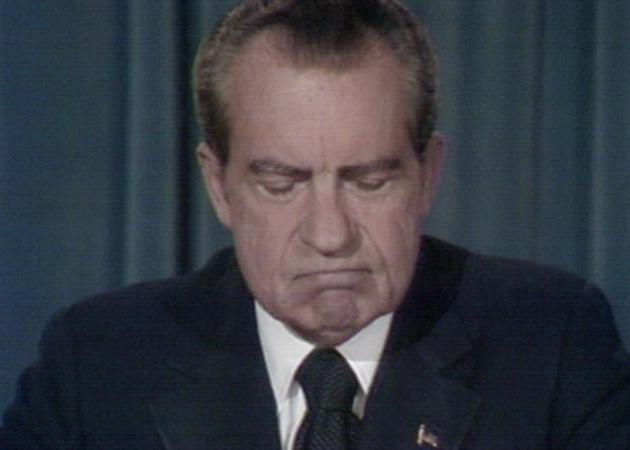
\includegraphics[width=.375\textwidth]{Images/NixonBad.jpeg}  \end{center} & \begin{center} 
\includegraphics[width=.175\textwidth]{Images/NixonGood.png}  \end{center}\\
    \hline
    \begin{itemize}
      \item The modern conservative movement is (indirectly) rooted in Nixon's presidency
      \item The events at the Watergate Hotel are a permanent, and most well known stain on Nixon's presidency
      \item Claimed to be anticommunist, but actively endorsed Communist China's relations with the US
    \end{itemize} &
    \begin{itemize}
      \item Nixon was able to semi-successfully deescalate the war in Vietnam
      \item Nixon lessened tensions with the USSR, and was able to create a period of relative piece:  det\'ente
      \item Nixon created the Environment Protection Agency (EPA), which still exists to this day
    \end{itemize}\\
    \hline
  \end{tabular}
\end{center}

\end{document}

